\documentclass[a4paper]{article}

\usepackage[english]{babel}
\usepackage[utf8]{inputenc}
\usepackage{amsmath}
\usepackage{float}
\usepackage{graphicx}
\usepackage[colorinlistoftodos]{todonotes}

\usepackage{geometry}
 \geometry{
 a4paper,
 total={170mm,257mm},
 left=20mm,
 top=20mm,
 }
 
\title{Report \#4}

\author{Ariel Soto Caro}

\date{\today}

\begin{document}
\maketitle

\section*{Pooled estimation}
In this case I just perform an estimation for the production function. The first model is the original one, the log for each input, and a trend, or a dummy per year. The Model 2 include just a categorical variable indicating if such firm experience an acquisition or a merging process. For example, if a specific firm $i$ experience a merge in year 1990, variable ``Acqu \& Merg'' is zero from 1986 to 1989 and is equal to one from 1990 to 1996. Finally, the Model 3 consider variable ``Acqu \& Merg'' also, and the log of prices. An interesting issue in this last model is the log of fuel prices is positive and is significant.

In the second page of this report can be observe one graph for each estimation. Model 1 and 2 are very similar (this can be observed in the table also, obviously). But the model 3 differ of the rest in 3 dimensions: (i) the Confidence Intervals are slightly more wide than the other models; (ii) the behavior of model with a dummy per year presents movements in opposite directions regards the previous models (e.g. year 1991) and ; (iii) probably because the former 2 reasons, there are more points inside the confidence interval than the previous models.



% Table generated by Excel2LaTeX from sheet 'Sheet1'
\begin{table}[H]
  \centering
  \caption{Estimation by OLS.}
    \begin{tabular}{lrlrlrlrlrlrl} \hline
          & \multicolumn{4}{c}{\textbf{Model 1}}   & \multicolumn{4}{c}{\textbf{Model 2}}   & \multicolumn{4}{c}{\textbf{Model 3}} \\ \hline
    \textit{Coefficients} & \multicolumn{2}{c}{\textit{with trend}} & \multicolumn{2}{c}{\textit{dummy p/year}} & \multicolumn{2}{c}{\textit{with trend}} & \multicolumn{2}{c}{\textit{dummy p/year}} & \multicolumn{2}{c}{\textit{with trend}} & \multicolumn{2}{c}{\textit{dummy p/year}} \\ \hline \hline
    (Intercept) & 5.071 & ***   & 5.031 & ***   & 5.098 & ***   & 5.055 & ***   & 4.992 & ***   & 4.697 & *** \\
    log(labor) & 0.192 & ***   & 0.193 & ***   & 0.195 & ***   & 0.195 & ***   & 0.172 & ***   & 0.174 & *** \\
    log(fuel) & 0.625 & ***   & 0.625 & ***   & 0.628 & ***   & 0.628 & ***   & 0.639 & ***   & 0.633 & *** \\
    log(capital) & 0.174 & ***   & 0.173 & ***   & 0.168 & ***   & 0.168 & ***   & 0.174 & ***   & 0.180 & *** \\
    trend & 0.015 & ***   &       &       & 0.014 & ***   &       &       & 0.026 & ***   &       &  \\
    year87 &       &       & 0.089 & *     &       &       & 0.088 & *     &       &       & 0.103 & ** \\
    year88 &       &       & 0.090 & *     &       &       & 0.089 & *     &       &       & 0.171 & *** \\
    year89 &       &       & 0.145 & ***   &       &       & 0.143 & ***   &       &       & 0.198 & *** \\
    year90 &       &       & 0.147 & ***   &       &       & 0.145 & ***   &       &       & 0.192 & *** \\
    year91 &       &       & 0.142 & ***   &       &       & 0.139 & ***   &       &       & 0.211 & *** \\
    year92 &       &       & 0.141 & ***   &       &       & 0.135 & ***   &       &       & 0.209 & *** \\
    year93 &       &       & 0.118 & **    &       &       & 0.113 & **    &       &       & 0.184 & *** \\
    year94 &       &       & 0.155 & ***   &       &       & 0.150 & ***   &       &       & 0.281 & *** \\
    year95 &       &       & 0.178 & ***   &       &       & 0.170 & ***   &       &       & 0.309 & *** \\
    year96 &       &       & 0.225 & ***   &       &       & 0.215 & ***   &       &       & 0.322 & *** \\
    Acqu \& Merg &       &       &       &       & 0.042 & *     & 0.042 & *     & 0.058 & *     & 0.059 & * \\
    log(laborP) &       &       &       &       &       &       &       &       & -0.248 & ***   & -0.244 & *** \\
    log(fuelP) &       &       &       &       &       &       &       &       & 0.530 & ***   & 0.519 & *** \\
    log(capitalP) &       &       &       &       &       &       &       &       & -0.208 & **    & -0.319 & *** \\ \hline
    $R^2$     & 0.933 &       & 0.934 &       & 0.933 &       & 0.934 &       & 0.940 &       & 0.940 &  \\
    F-stat     & 3138.39 & ***   & 969   & ***   & 2516.73 & ***   & 901.9 & ***   & 1772.910 & ***   & 843.500 & *** \\ \hline
    \end{tabular}%
  \label{tab:addlabel}%
\end{table}%


\newpage


\begin{figure}[H]
\caption{Model 1.}
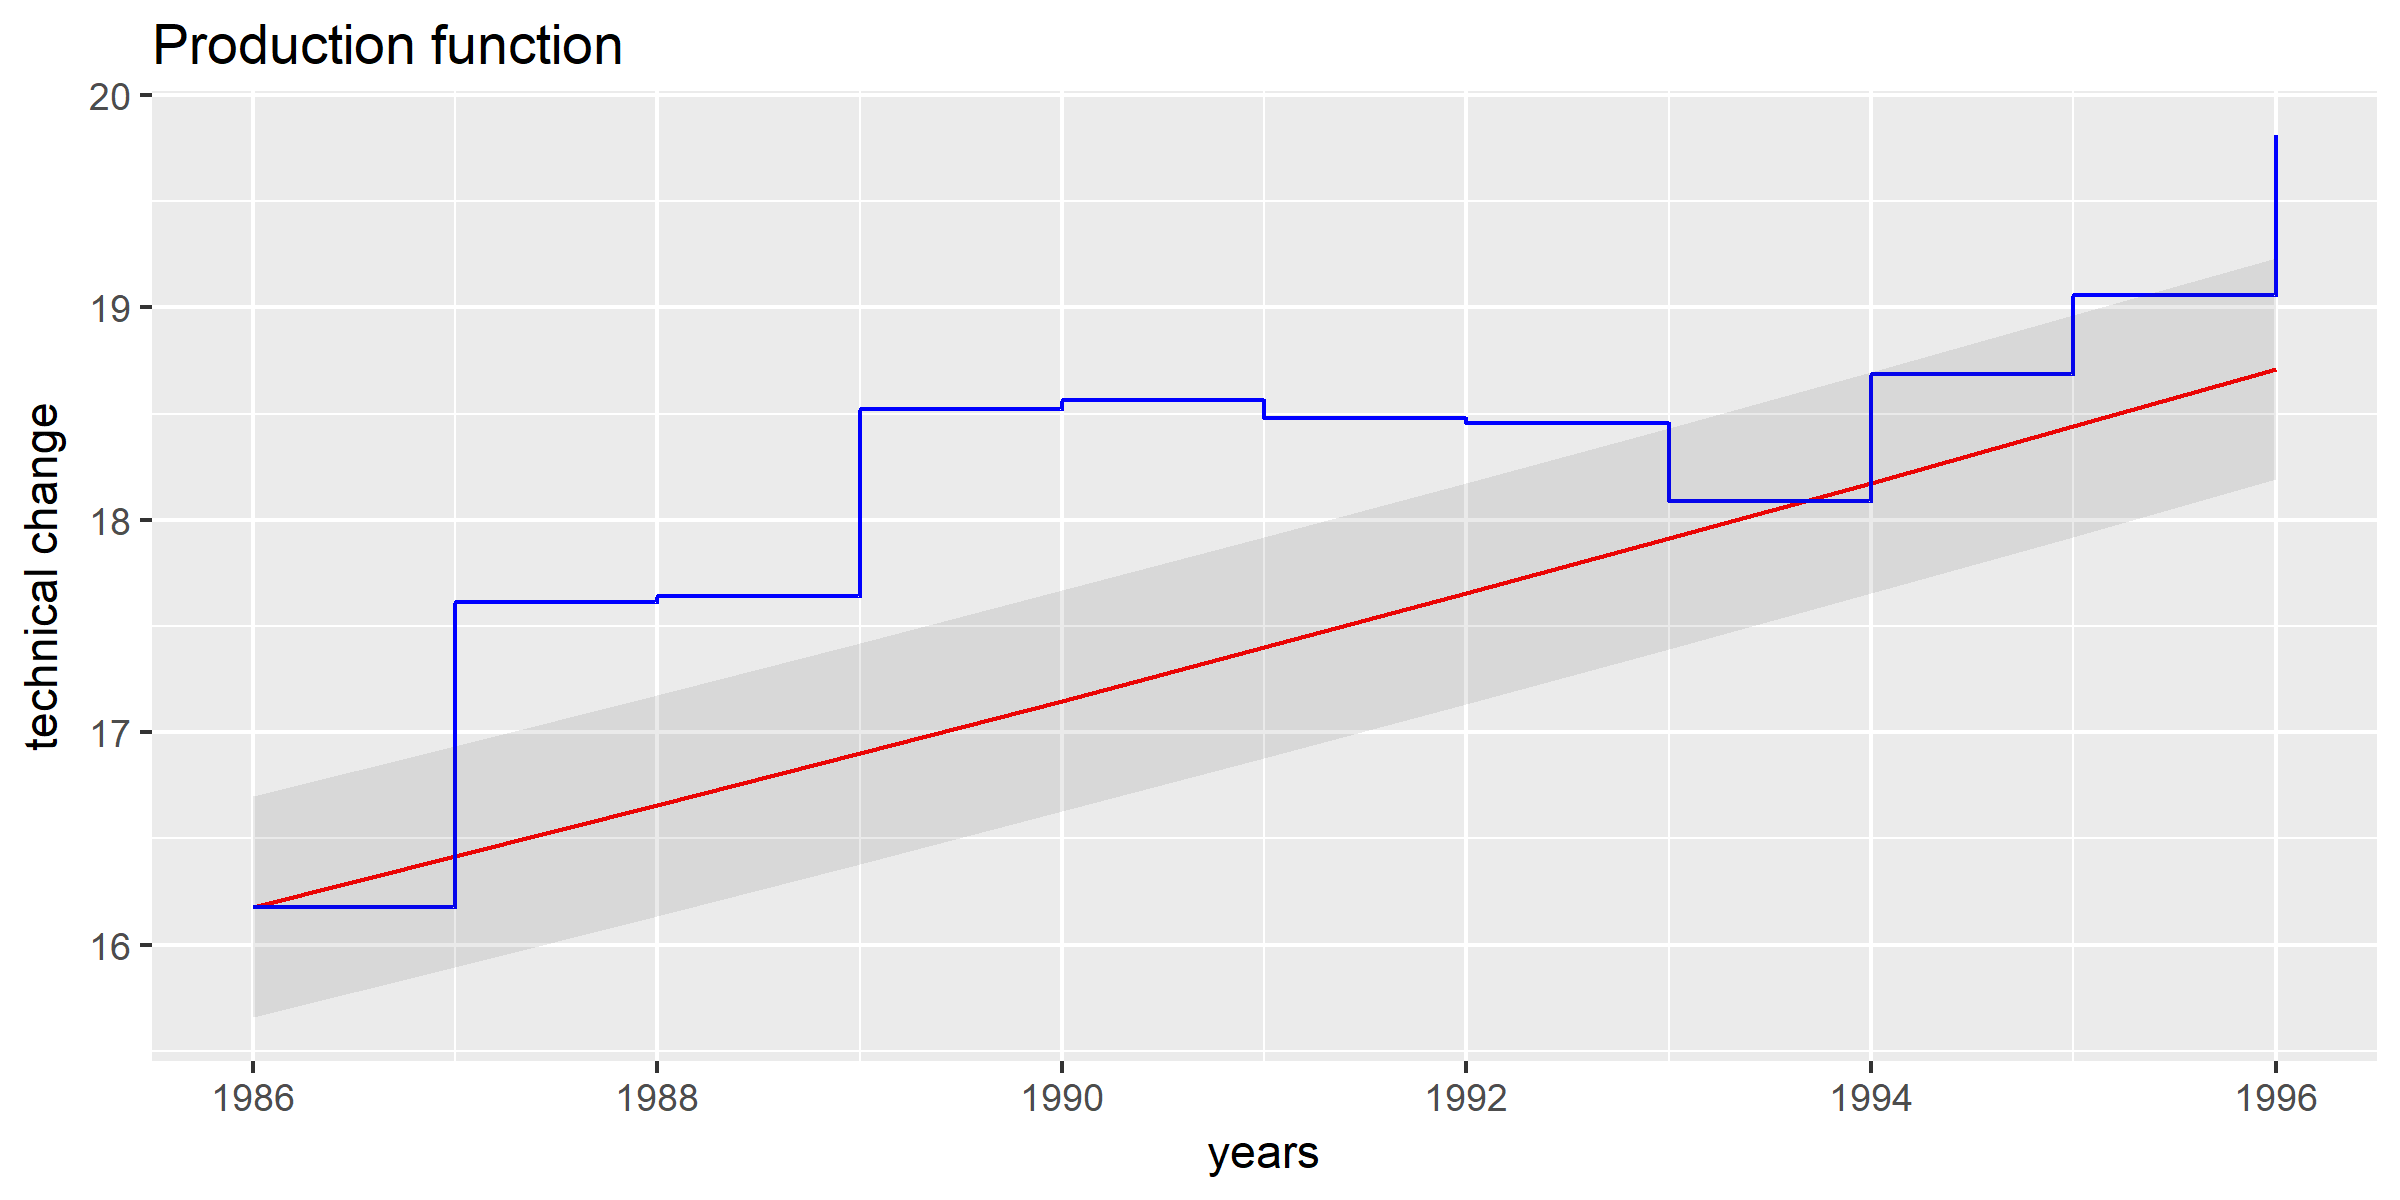
\includegraphics[scale=.70]{Prod_ols}
\end{figure}

\begin{figure}[H]
\caption{Model 2.}
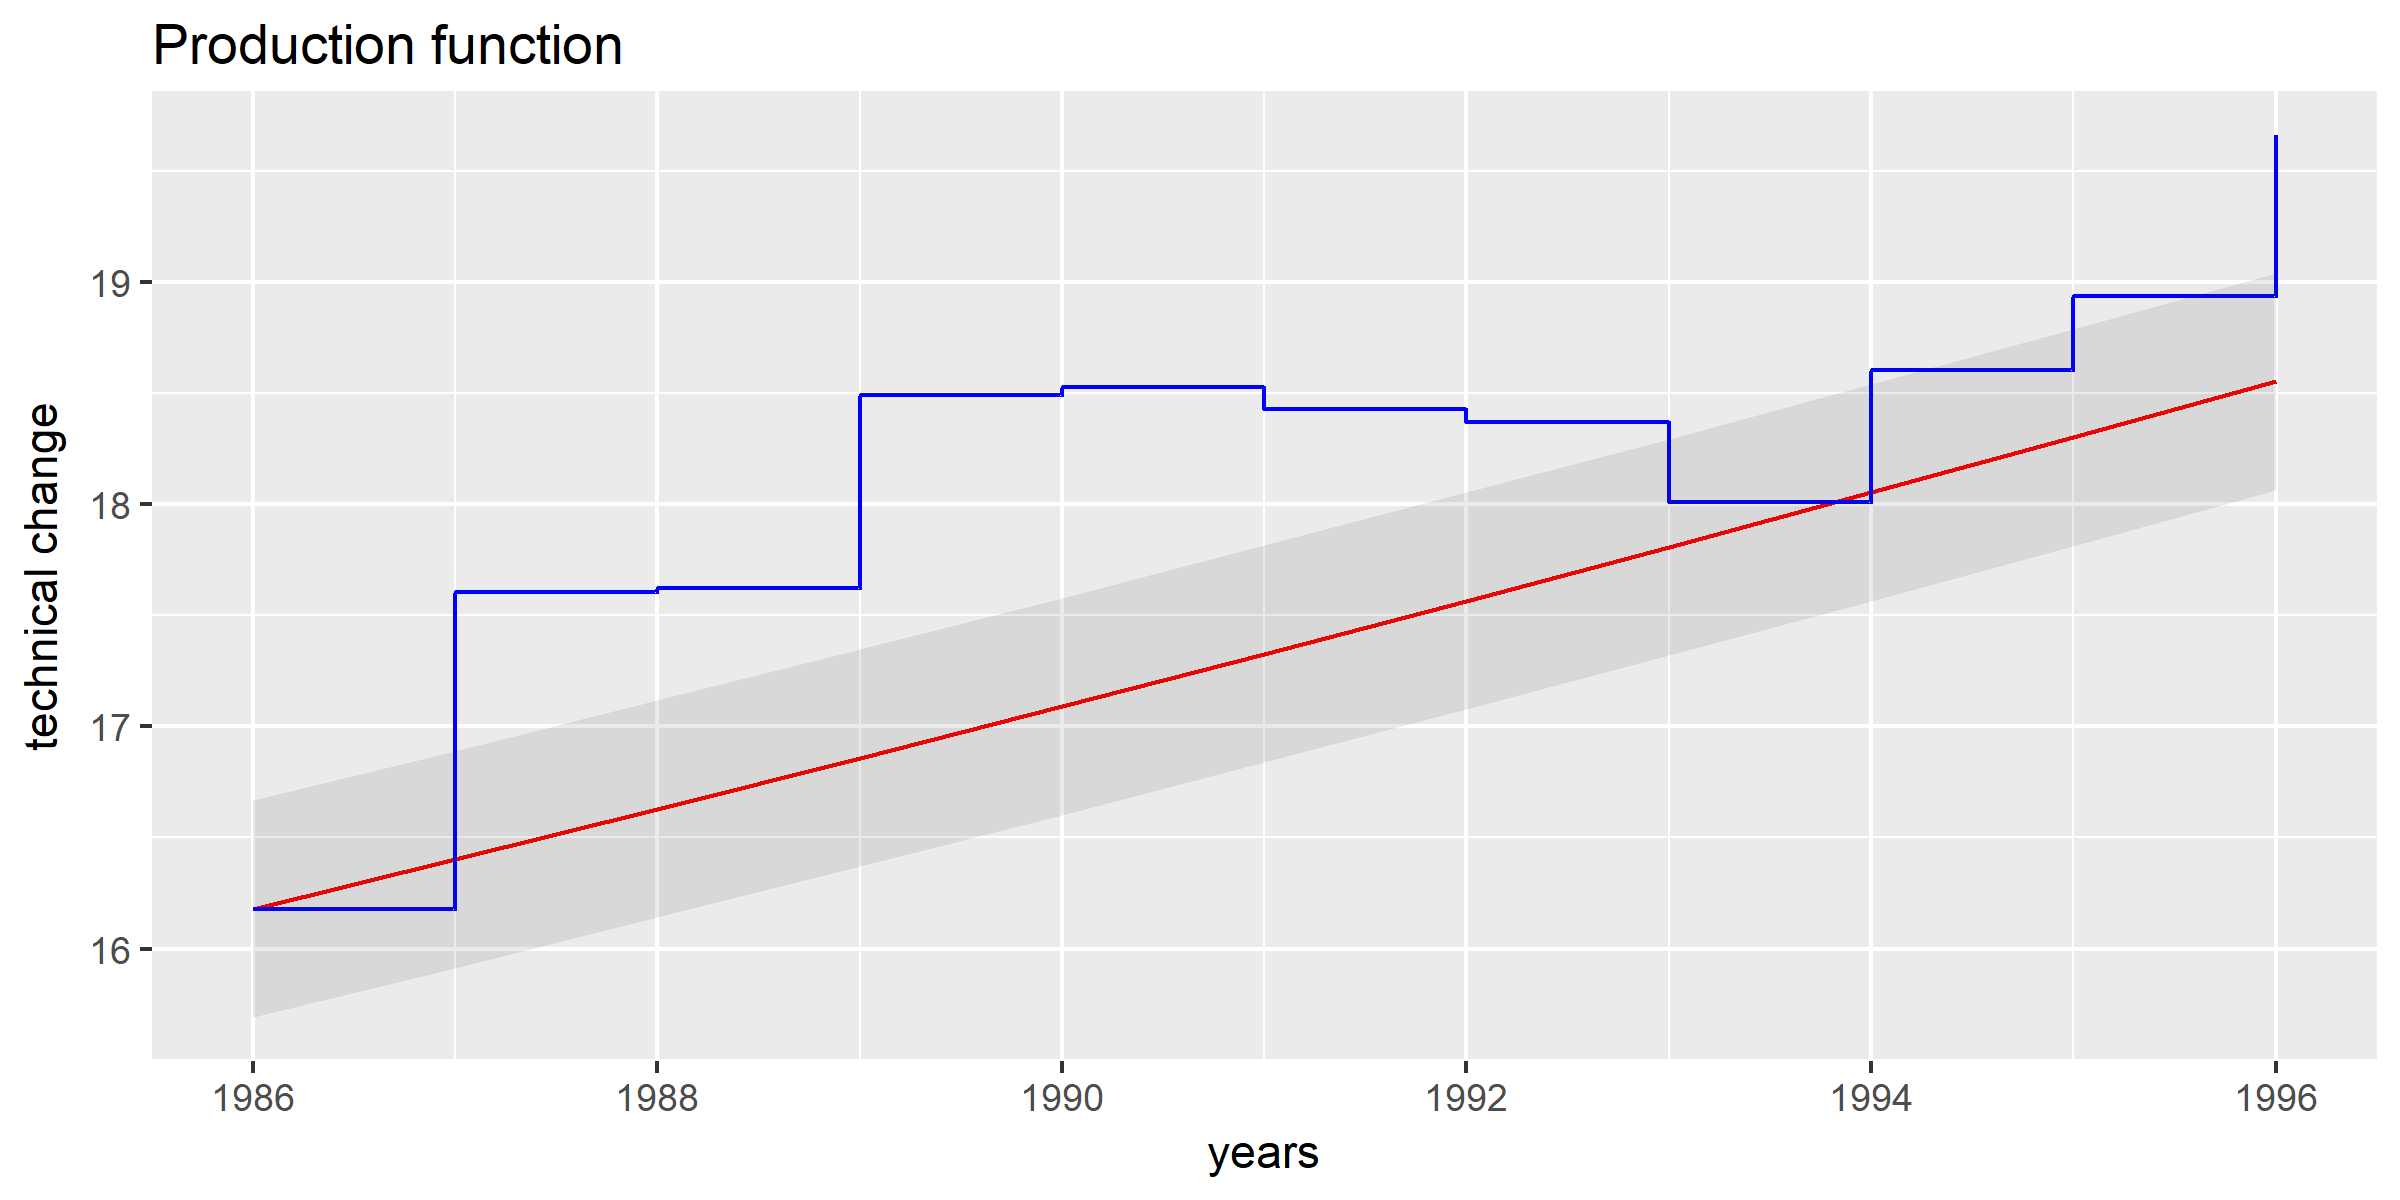
\includegraphics[scale=.70]{Prod_ols_model2}
\end{figure}

\begin{figure}[H]
\caption{Model 3.}
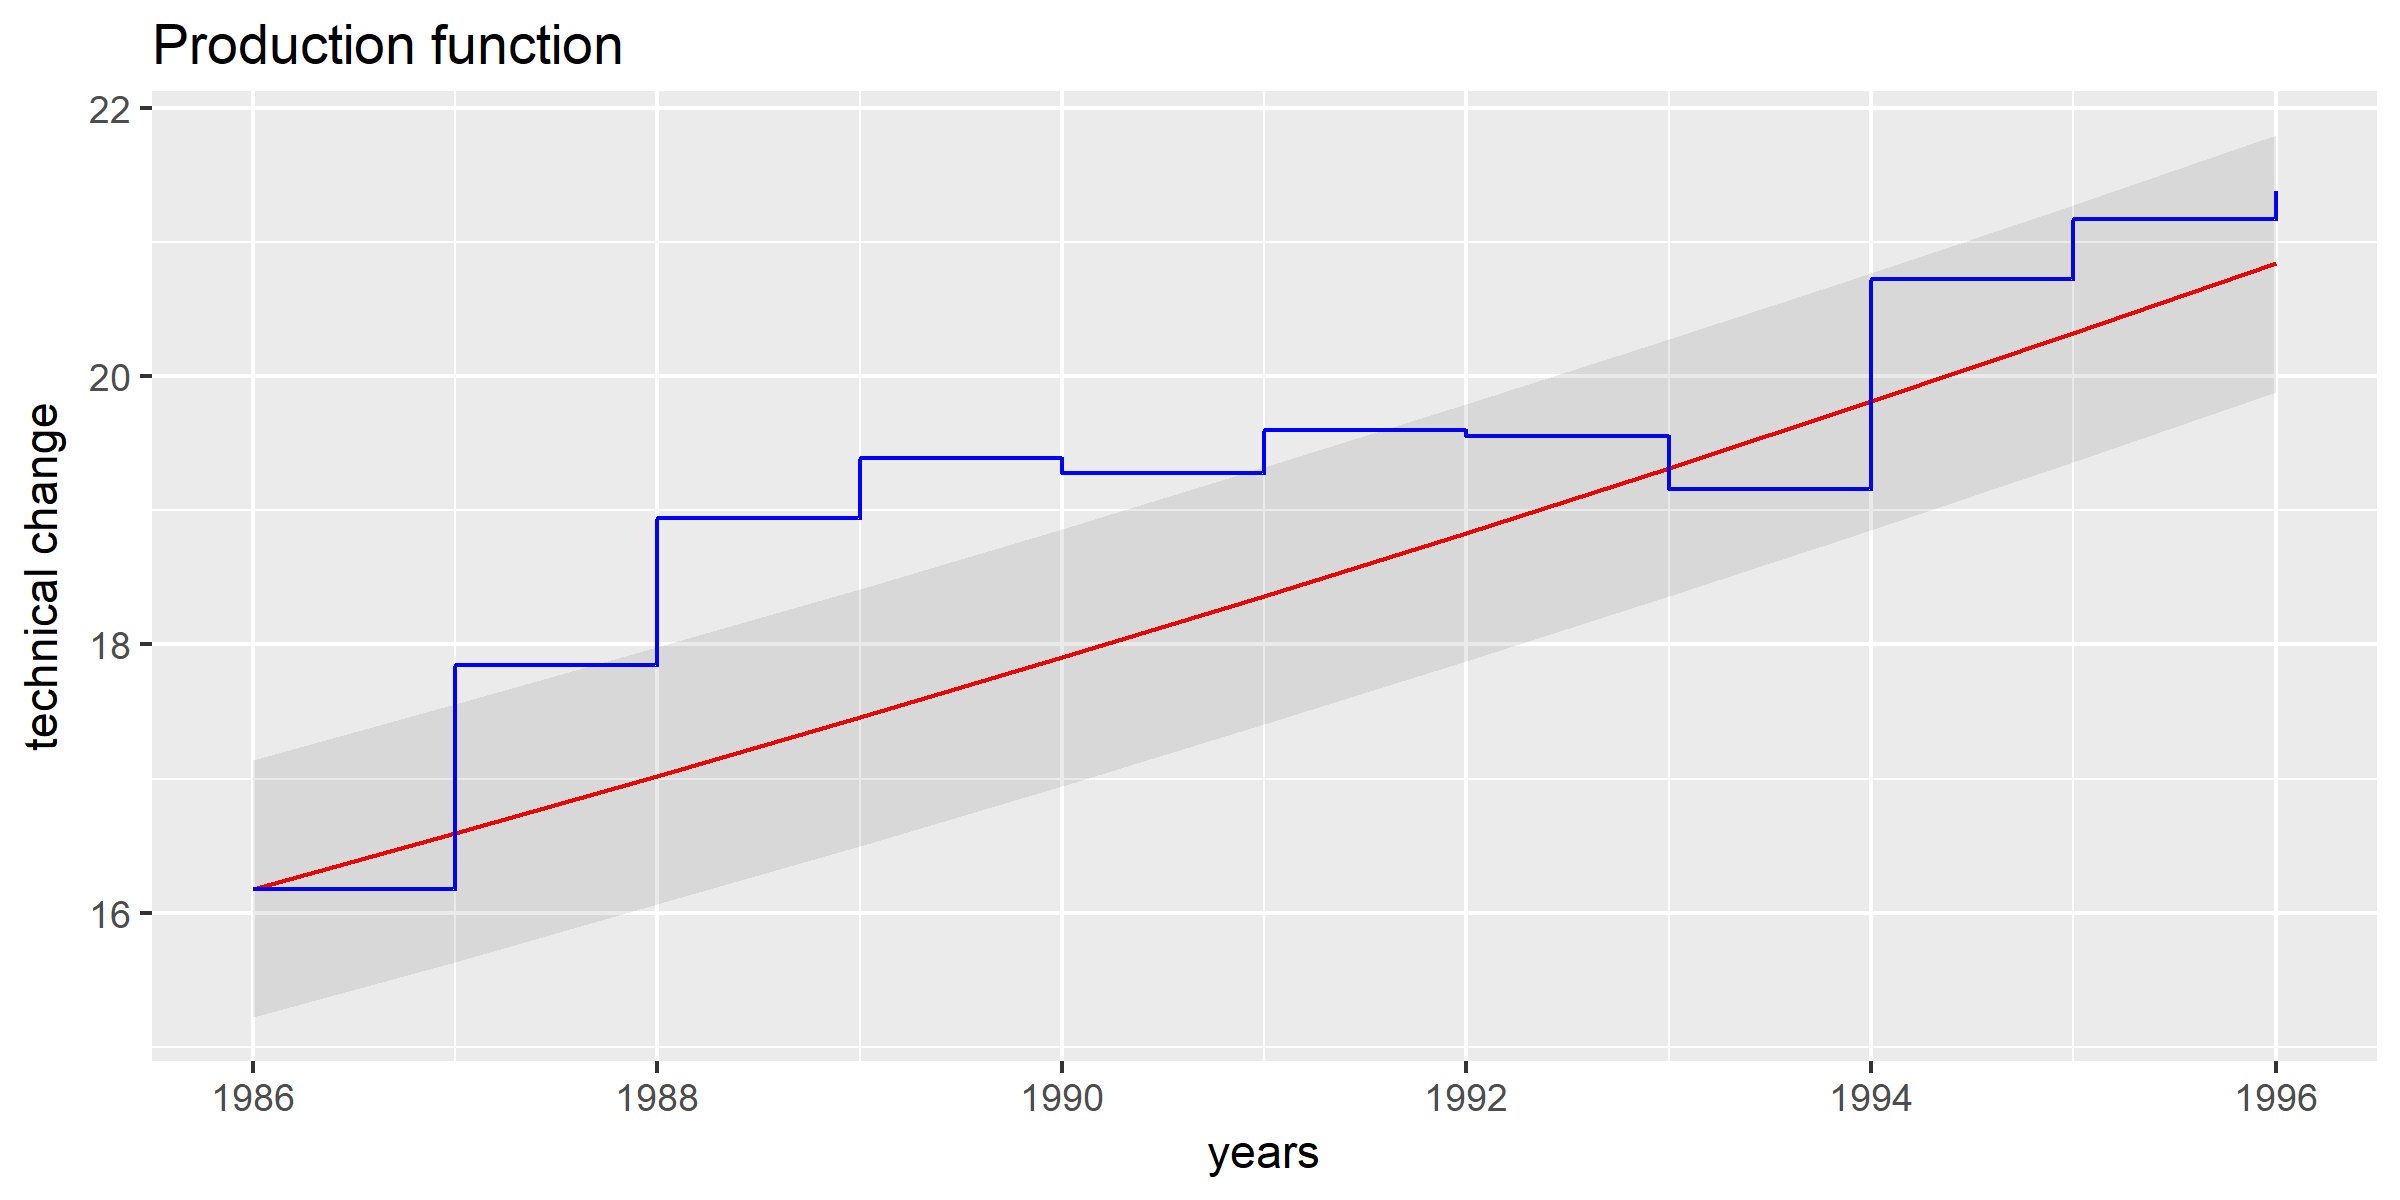
\includegraphics[scale=.70]{Prod_ols_model3}
\end{figure}


\end{document}